% !TeX root = ../main.tex
\chapter{Unidad 3: Fundamentos de la mecánica ondulatoria}
\label{chap:unidad-3}

\section{Propósito y resultados de aprendizaje}
\label{sec:u3-proposito}

Esta unidad estudia dos fenómenos relacionados, pero diferentes: la
\textbf{oscilación} de un sistema alrededor de una posición de equilibrio y la
\textbf{propagación} de una perturbación a través de un medio. La distinción
permite describir cómo se mueve el cono de un parlante, cómo oscilan localmente
las partículas del aire y cómo una onda sonora avanza desde la fuente hasta un
receptor sin transportar esas partículas junto con ella.

Al finalizar la unidad se espera que sea posible:

\begin{itemize}
    \item distinguir movimiento oscilatorio de movimiento ondulatorio;
    \item describir posición, velocidad y aceleración en un movimiento
    armónico simple;
    \item relacionar frecuencia, período y frecuencia angular, con sus
    unidades correspondientes;
    \item interpretar amplitud, fase inicial y diferencia de fase sin
    confundirlas con atributos perceptuales;
    \item leer una representación temporal y una representación espacial de
    una onda;
    \item calcular la longitud de onda a partir de la frecuencia y de la
    velocidad de propagación;
    \item diferenciar velocidad de partícula y velocidad de propagación;
    \item reconocer ondas longitudinales y transversales;
    \item aplicar el principio de superposición a casos de interferencia
    constructiva, parcial y destructiva;
    \item relacionar estos modelos con la generación de un tono mediante un
    parlante y con el uso introductorio de tonos en Fonoaudiología.
\end{itemize}

\section{Conocimientos previos}
\label{sec:u3-previos}

Se utilizarán la función seno y la función coseno, los radianes, la conversión
de unidades y el análisis dimensional introducidos en la
Unidad~\ref{chap:unidad-1}. De la Unidad~\ref{chap:unidad-2} se retomarán la
posición de equilibrio, la inercia, la fuerza restauradora, el modelo
masa--resorte y la diferencia entre velocidad local y velocidad de
propagación. No se requiere desarrollar cálculo diferencial: las expresiones
de velocidad y aceleración se interpretarán como tasas de cambio de la
posición y de la velocidad.

\section{De la oscilación local a la onda}
\label{sec:u3-oscilacion-onda}

\subsection{Movimiento oscilatorio}
\label{sec:u3-movimiento-oscilatorio}

Un sistema presenta \textbf{movimiento oscilatorio} cuando se desplaza a un
lado y al otro de una posición de equilibrio. El movimiento corresponde a un
sistema localizado: puede oscilar una masa unida a un resorte, el extremo de
un diapasón, una porción de una membrana o el cono de un parlante.

La posición de equilibrio no tiene que coincidir con la coordenada cero
elegida en cualquier sistema de referencia. Para simplificar el modelo,
adoptaremos como origen esa posición y representaremos mediante \(x\) el
\textbf{desplazamiento}, medido en metros (\(\text{m}\)). Un valor \(x>0\)
indica desplazamiento en el sentido elegido como positivo; un valor \(x<0\)
indica desplazamiento en el sentido contrario.

Una oscilación no es necesariamente periódica ni armónica. Puede disminuir por
amortiguamiento, variar de un ciclo a otro o resultar de varias componentes.
El movimiento armónico simple, que se estudiará en la
sección~\ref{sec:u3-mas}, es un modelo ideal particular.

\subsection{Movimiento ondulatorio}
\label{sec:u3-movimiento-ondulatorio}

Una \textbf{onda mecánica} aparece cuando una perturbación se propaga mediante
la interacción entre regiones vecinas de un medio material. Cada región puede
moverse alrededor de su posición de equilibrio y transmitir la perturbación a
la siguiente. La perturbación y la energía asociada avanzan, pero, en el
modelo ondulatorio ideal, no existe un transporte neto de materia desde la
fuente hasta el receptor.

Esta descripción reúne dos escalas de movimiento:

\begin{itemize}
    \item el \textbf{movimiento local} de una partícula o de una pequeña
    región del medio;
    \item la \textbf{propagación} del estado de perturbación a través del
    medio.
\end{itemize}

Por ejemplo, una compresión producida en un resorte largo puede avanzar varios
metros mientras una espira marcada se desplaza solo una distancia pequeña
alrededor de su posición de equilibrio. En el aire sucede algo análogo: las
partículas oscilan localmente y las variaciones mecánicas se propagan.

La figura~\ref{fig:u3-oscilacion-propagacion} compara dos instantes del
proceso. La región marcada cambia de posición alrededor de su equilibrio,
mientras la zona comprimida avanza una distancia mucho mayor.

\begin{figure}[htbp]
    \centering
    % Propósito: distinguir el desplazamiento local de una región del medio del
% avance de una perturbación longitudinal.
% Origen: descripción cualitativa de las secciones
% \ref{sec:u3-movimiento-ondulatorio} y \ref{sec:u3-actividad-onda}.
% Esquema conceptual, no representa datos medidos ni está dibujado a escala.
% Descripción accesible: dos instantes de una hilera de partículas. La misma
% partícula marcada permanece cerca de su posición de equilibrio, mientras una
% región de compresión se desplaza desde la izquierda hacia la derecha.
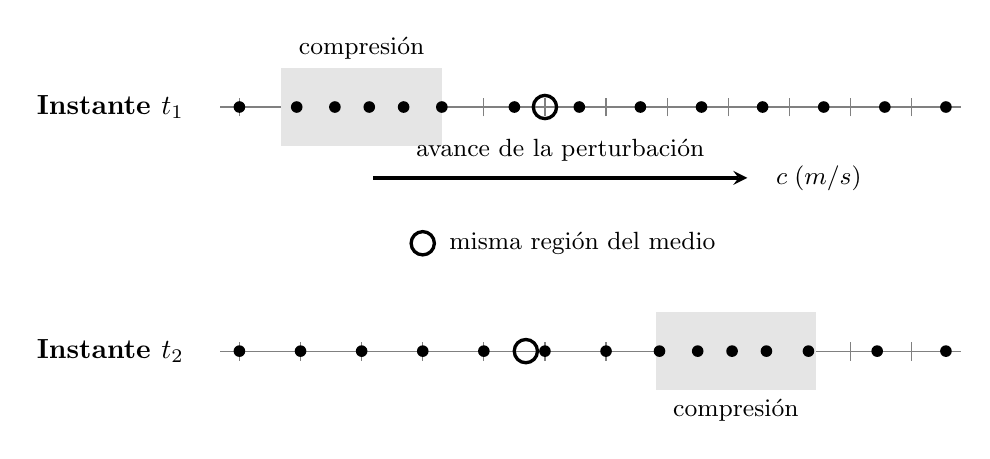
\begin{tikzpicture}[font=\small,>=stealth,x=0.97cm,y=1cm]
    \node[anchor=east,font=\bfseries] at (1.2,1.55) {Instante \(t_1\)};
    \node[anchor=east,font=\bfseries] at (1.2,-1.55) {Instante \(t_2\)};

    % Posiciones de equilibrio.
    \foreach \y in {1.55,-1.55}{
        \draw[gray] (1.55,\y) -- (11.25,\y);
        \foreach \x in {1.8,2.6,...,11.0}{
            \draw[gray] (\x,\y-0.12) -- (\x,\y+0.12);
        }
    }

    % Regiones comprimidas en dos posiciones diferentes.
    \fill[black!10] (2.35,1.05) rectangle (4.45,2.05);
    \fill[black!10] (7.25,-2.05) rectangle (9.35,-1.05);
    \node at (3.40,2.30) {compresión};
    \node at (8.30,-2.30) {compresión};

    % Partículas en t1.
    \foreach \x in {1.8,2.55,3.05,3.50,3.95,4.45,5.40,6.25,7.05,7.85,8.65,9.45,10.25,11.05}{
        \fill (\x,1.55) circle (2.1pt);
    }
    % Partículas en t2.
    \foreach \x in {1.8,2.60,3.40,4.20,5.00,5.80,6.60,7.30,7.80,8.25,8.70,9.25,10.15,11.05}{
        \fill (\x,-1.55) circle (2.1pt);
    }

    % Misma región del medio, marcada en ambos instantes.
    \draw[very thick] (5.80,1.55) circle (4.2pt);
    \draw[very thick] (5.55,-1.55) circle (4.2pt);
    \draw[very thick] (4.20,-0.18) circle (4.2pt);
    \node[anchor=west,align=left] at (4.42,-0.18)
        {misma región del medio};

    % Avance de la perturbación.
    \draw[->,very thick] (3.55,0.65) -- (8.45,0.65)
        node[midway,above=2pt] {avance de la perturbación};
    \node[anchor=west,align=left] at (8.70,0.65)
        {\(c\;(\text{m}/\text{s})\)};
\end{tikzpicture}

    \caption{Movimiento local y propagación en una onda longitudinal
    esquemática. La misma región del medio permanece cerca de su posición de
    equilibrio, aunque la compresión avance con velocidad \(c\). Elaboración
    propia; el dibujo no está a escala.}
    \label{fig:u3-oscilacion-propagacion}
\end{figure}

\subsection{Ondas longitudinales y transversales}
\label{sec:u3-longitudinal-transversal}

El tipo de onda se determina comparando la dirección del movimiento local con
la dirección de propagación:

\begin{description}
    \item[\textbf{Onda longitudinal:}] el movimiento local ocurre en una
    dirección paralela a la propagación. En gases y líquidos, el sonido se
    describe mediante compresiones y rarefacciones y es longitudinal.
    \item[\textbf{Onda transversal:}] el movimiento local ocurre en una
    dirección perpendicular a la propagación. Una onda en una cuerda tensa
    constituye un ejemplo introductorio.
\end{description}

Los sólidos pueden admitir ondas longitudinales y transversales porque pueden
resistir deformaciones de compresión y de corte. Esta clasificación no debe
utilizarse para reducir la audición por vía ósea a un único tipo de onda: sus
mecanismos se estudiarán en la unidad dedicada al sistema auditivo.

La figura~\ref{fig:u3-longitudinal-transversal} hace explícita la comparación
geométrica que define ambos tipos de onda. Las curvas o hileras dibujadas son
esquemas del movimiento del medio, no atributos perceptuales.

\begin{figure}[htbp]
    \centering
    % Propósito: clasificar una onda comparando la dirección del movimiento local
% con la dirección de propagación.
% Origen: definiciones de la sección \ref{sec:u3-longitudinal-transversal}.
% Esquema conceptual, no representa datos medidos ni está dibujado a escala.
% Descripción accesible: en el panel superior, las partículas de una onda
% longitudinal se desplazan horizontalmente, en paralelo a la propagación. En
% el panel inferior, una cuerda se desplaza verticalmente mientras la onda se
% propaga horizontalmente.
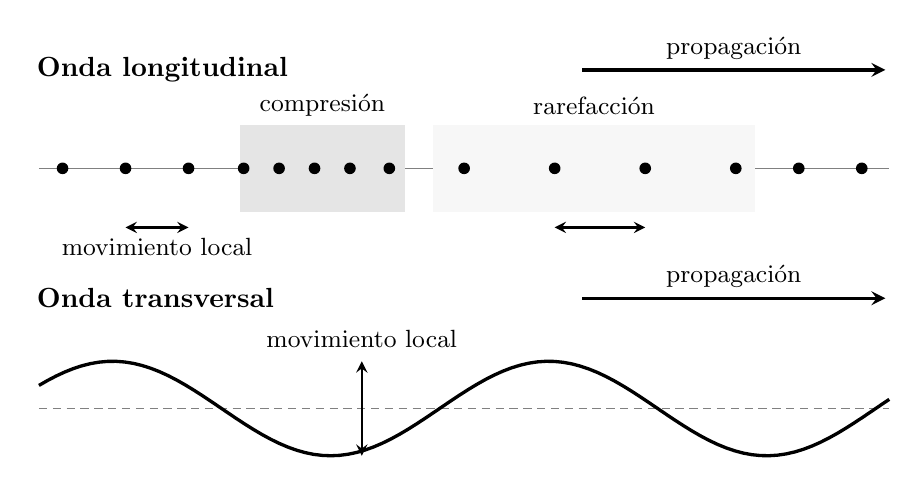
\begin{tikzpicture}[font=\small,>=stealth,x=1cm,y=1cm]
    \node[anchor=west,font=\bfseries] at (0.3,2.10)
        {Onda longitudinal};
    \draw[->,very thick] (7.35,2.10) -- (11.20,2.10)
        node[midway,above] {propagación};

    \draw[gray] (0.45,0.85) -- (11.25,0.85);
    \fill[black!10] (3.00,0.30) rectangle (5.10,1.40);
    \fill[black!3] (5.45,0.30) rectangle (9.55,1.40);
    \node at (4.05,1.65) {compresión};
    \node at (7.50,1.65) {rarefacción};
    \foreach \x in {0.75,1.55,2.35,3.05,3.50,3.95,4.40,4.90,5.85,7.00,8.15,9.30,10.10,10.90}{
        \fill (\x,0.85) circle (2.1pt);
    }
    \draw[<->,thick] (1.55,0.10) -- (2.35,0.10)
        node[midway,below] {movimiento local};
    \draw[<->,thick] (7.00,0.10) -- (8.15,0.10);

    \node[anchor=west,font=\bfseries] at (0.3,-0.80)
        {Onda transversal};
    \draw[->,very thick] (7.35,-0.80) -- (11.20,-0.80)
        node[midway,above] {propagación};
    \draw[densely dashed,gray] (0.45,-2.20) -- (11.25,-2.20);
    \draw[very thick,samples=100,domain=0.45:11.25]
        plot (\x,{-2.20+0.60*sin(65*\x)});
    \draw[<->,thick] (4.55,-2.80) -- (4.55,-1.60);
    \node[above] at (4.55,-1.55) {movimiento local};
\end{tikzpicture}

    \caption{Clasificación según la dirección del movimiento local. En una
    onda longitudinal, el movimiento es paralelo a la propagación; en una
    onda transversal, es perpendicular. Elaboración propia; esquema
    cualitativo y no a escala.}
    \label{fig:u3-longitudinal-transversal}
\end{figure}

\subsection{Actividad de observación}
\label{sec:u3-actividad-onda}

Puede colocarse un resorte largo sobre una mesa y marcar una espira con una
cinta liviana. Al producir un pulso pequeño en la dirección del resorte se
observa por separado:

\begin{enumerate}
    \item el desplazamiento limitado de la espira marcada;
    \item el avance de la zona comprimida;
    \item la diferencia entre la distancia recorrida por la perturbación y la
    distancia recorrida por la espira.
\end{enumerate}

La actividad no reproduce todos los detalles de una onda acústica, pero
permite distinguir visualmente movimiento local y propagación.

\section{Movimiento armónico simple}
\label{sec:u3-mas}

\subsection{Interpretación física}
\label{sec:u3-mas-interpretacion}

En el modelo masa--resorte de la Unidad~\ref{chap:unidad-2}, una fuerza
restauradora lineal apunta hacia la posición de equilibrio. Si se omiten por
el momento el amortiguamiento y la fuerza externa, la fuerza elástica es
\(F_\mathrm{el}=-kx\), donde \(k\) es la rigidez, medida en newtons por metro
(\(\text{N}/\text{m}\)), y \(x\) es el desplazamiento, medido en metros.

Al combinar esa fuerza con la segunda ley de Newton se obtiene:

\begin{equation}
    ma=-kx,
    \label{eq:u3-mas-fuerza}
\end{equation}

donde \(m\) es la masa, medida en kilogramos (\(\text{kg}\)), y \(a\) es la
aceleración, medida en metros por segundo cuadrado
(\(\text{m}/\text{s}^{2}\)). La ecuación~\eqref{eq:u3-mas-fuerza} muestra la
idea central: cuanto más se aleja el sistema del equilibrio, mayor es la
aceleración dirigida hacia él.

Este movimiento se denomina \textbf{movimiento armónico simple} (MAS). El
modelo supone una fuerza restauradora proporcional al desplazamiento. Un
péndulo, por ejemplo, puede aproximarse mediante un MAS solo para oscilaciones
angulares pequeñas; no todo movimiento de vaivén es armónico simple.

\subsection{Amplitud, frecuencia, período y fase inicial}
\label{sec:u3-parametros-mas}

Antes de escribir la ecuación temporal se definen sus magnitudes:

\begin{description}
    \item[\textbf{Amplitud (\(A\)):}] en este modelo es el máximo valor
    absoluto del desplazamiento respecto del equilibrio y se mide en metros
    (\(\text{m}\)).
    \item[\textbf{Frecuencia (\(f\)):}] número de ciclos por unidad de tiempo.
    Se mide en hertz (\(\text{Hz}\)), donde
    \(1\,\text{Hz}=1\,\text{s}^{-1}\).
    \item[\textbf{Período (\(T\)):}] tiempo necesario para completar un ciclo.
    Se mide en segundos (\(\text{s}\)).
    \item[\textbf{Frecuencia angular (\(\omega\)):}] rapidez con la que cambia
    la fase de la oscilación. Se mide en radianes por segundo
    (\(\text{rad}/\text{s}\)).
    \item[\textbf{Fase inicial (\(\varphi_0\)):}] estado del ciclo en
    \(t=0\). Se expresa en radianes (\(\text{rad}\)).
\end{description}

Frecuencia, período y frecuencia angular se relacionan mediante:

\begin{equation}
    T=\frac{1}{f},
    \qquad
    \omega=2\pi f=\frac{2\pi}{T}.
    \label{eq:u3-f-t-omega}
\end{equation}

Para el sistema masa--resorte ideal de la
ecuación~\eqref{eq:u3-mas-fuerza}, la frecuencia angular propia también
satisface:

\begin{equation}
    \omega=\sqrt{\frac{k}{m}},
    \label{eq:u3-omega-masa-resorte}
\end{equation}

donde \(k\) se mide en \(\text{N}/\text{m}\) y \(m\) en
\(\text{kg}\). Esta relación pertenece al modelo lineal sin amortiguamiento
ni fuerza externa; un sistema real puede requerir una descripción más
completa.

Definidas estas magnitudes, el desplazamiento temporal del MAS puede
escribirse como:

\begin{equation}
    x(t)=A\cos\left(\omega t+\varphi_0\right),
    \label{eq:u3-mas-posicion}
\end{equation}

donde \(t\) es el tiempo, medido en segundos. El argumento
\(\omega t+\varphi_0\) es una fase y, por lo tanto, es adimensional; el radián
se conserva para indicar su interpretación angular. La ecuación describe la
posición de un sistema a lo largo del tiempo, no la forma espacial de una
onda.

La fase inicial no modifica la amplitud, la frecuencia ni el período. Solo
establece qué parte del ciclo corresponde al instante elegido como
\(t=0\). Por ejemplo, con \(\varphi_0=0\), la función coseno comienza en
\(x(0)=A\); con \(\varphi_0=\pi/2\,\text{rad}\), comienza en \(x(0)=0\) y el
movimiento inicial ocurre hacia valores negativos de \(x\).

\subsection{Posición, velocidad y aceleración}
\label{sec:u3-posicion-velocidad-aceleracion}

La \textbf{velocidad} informa cuánto cambia la posición por unidad de tiempo y
se mide en metros por segundo (\(\text{m}/\text{s}\)). Para el MAS de la
ecuación~\eqref{eq:u3-mas-posicion}:

\begin{equation}
    v(t)=-\omega A\sin\left(\omega t+\varphi_0\right).
    \label{eq:u3-mas-velocidad}
\end{equation}

Su valor absoluto máximo es:

\begin{equation}
    v_{\max}=\omega A=2\pi fA.
    \label{eq:u3-velocidad-maxima}
\end{equation}

La \textbf{aceleración} informa cuánto cambia la velocidad por unidad de
tiempo y se mide en metros por segundo cuadrado
(\(\text{m}/\text{s}^{2}\)). En el mismo modelo:

\begin{equation}
    a(t)=-\omega^{2}A\cos\left(\omega t+\varphi_0\right)
        =-\omega^{2}x(t).
    \label{eq:u3-mas-aceleracion}
\end{equation}

Estas expresiones permiten interpretar el ciclo:

\begin{itemize}
    \item en los extremos, \(x=\pm A\), la velocidad es cero y la aceleración
    apunta hacia el equilibrio;
    \item al pasar por el equilibrio, \(x=0\), la aceleración es cero y el
    valor absoluto de la velocidad es máximo;
    \item posición, velocidad y aceleración varían con la misma frecuencia,
    pero no alcanzan sus máximos en el mismo instante.
\end{itemize}

La figura~\ref{fig:u3-mas-cinematica} normaliza cada magnitud por su valor
máximo para comparar las fases sin mezclar metros, metros por segundo y metros
por segundo cuadrado. Los valores físicos se recuperan multiplicando cada
curva por \(A\), \(\omega A\) o \(\omega^{2}A\), respectivamente.

\begin{figure}[htbp]
    \centering
    % Propósito: relacionar el estado físico de un oscilador con las fases de su
% posición, velocidad y aceleración.
% Origen: x/A=cos(2 pi t/T), v/(omega A)=-sin(2 pi t/T) y
% a/(omega^2 A)=-cos(2 pi t/T), ecuaciones
% \eqref{eq:u3-mas-posicion}, \eqref{eq:u3-mas-velocidad} y
% \eqref{eq:u3-mas-aceleracion}, con fase inicial igual a cero.
% Curvas teóricas normalizadas; no representan datos medidos.
% Descripción accesible: arriba se muestra una masa en el extremo positivo,
% con aceleración hacia el equilibrio. Debajo, tres gráficos normalizados
% muestran que posición y aceleración tienen signos opuestos, y que la
% velocidad es máxima al pasar por el equilibrio.
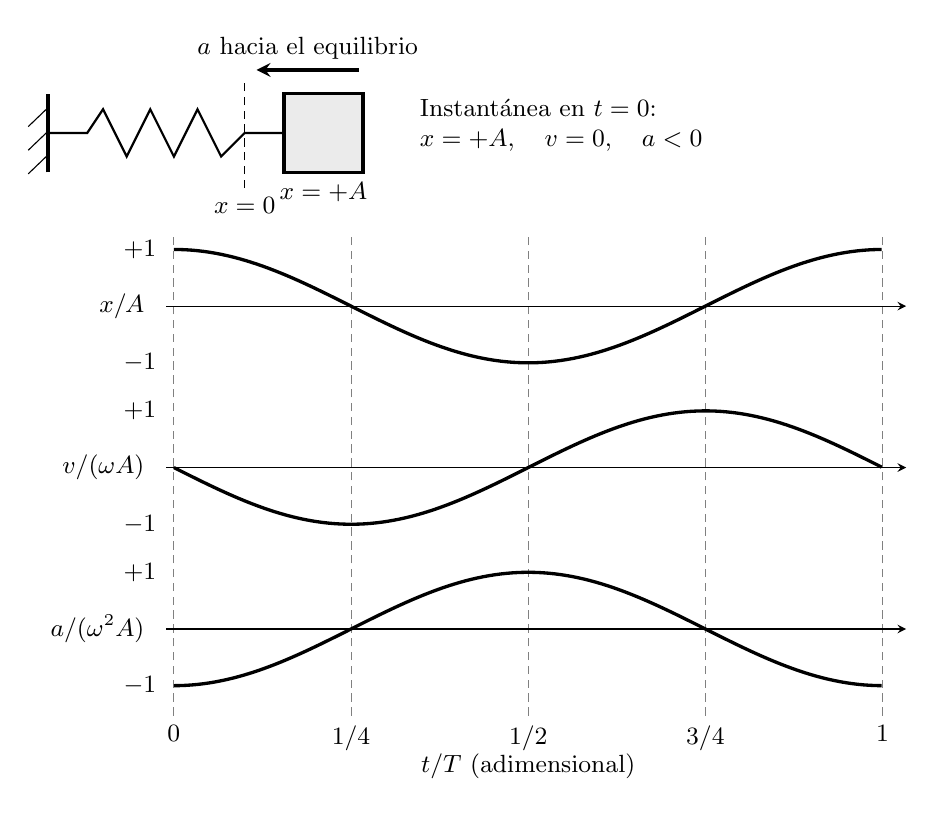
\begin{tikzpicture}[font=\small,>=stealth,x=1cm,y=1cm]
    % Instantánea física correspondiente a t=0.
    \draw[very thick] (0.55,3.75) -- (0.55,4.75);
    \foreach \y in {3.85,4.15,4.45}{
        \draw (0.30,\y-0.12) -- (0.55,\y+0.12);
    }
    \draw[thick] (0.55,4.25) -- (1.05,4.25)
        -- (1.25,4.55) -- (1.55,3.95)
        -- (1.85,4.55) -- (2.15,3.95)
        -- (2.45,4.55) -- (2.75,3.95)
        -- (3.05,4.25) -- (3.55,4.25);
    \draw[very thick,fill=black!8] (3.55,3.75) rectangle (4.55,4.75);
    \draw[densely dashed] (3.05,3.55) -- (3.05,4.95);
    \node[below] at (3.05,3.55) {\(x=0\)};
    \node[below] at (4.05,3.75) {\(x=+A\)};
    \draw[->,very thick] (4.50,5.05) -- (3.20,5.05)
        node[midway,above] {\(a\) hacia el equilibrio};
    \node[anchor=west,align=left] at (5.15,4.35)
        {Instantánea en \(t=0\):\\\(x=+A,\quad v=0,\quad a<0\)};

    % Escalas comunes de tiempo normalizado.
    \foreach \q/\lab in {0/{0},0.25/{1/4},0.5/{1/2},0.75/{3/4},1/{1}}{
        \pgfmathsetmacro{\xx}{2.15+9.0*\q}
        \draw[densely dashed,gray] (\xx,-3.15) -- (\xx,2.95);
        \node[below] at (\xx,-3.15) {\(\lab\)};
    }

    % Ejes horizontales de las tres magnitudes.
    \foreach \yy in {2.05,0,-2.05}{
        \draw[->] (2.05,\yy) -- (11.45,\yy);
    }
    \node[anchor=east] at (1.90,2.05) {\(x/A\)};
    \node[anchor=east] at (1.90,0) {\(v/(\omega A)\)};
    \node[anchor=east] at (1.90,-2.05) {\(a/(\omega^{2}A)\)};
    \node at (6.65,-3.80) {\(t/T\) (adimensional)};

    % Curvas normalizadas.
    \draw[very thick,samples=120,domain=0:1]
        plot ({2.15+9.0*\x},{2.05+0.72*cos(360*\x)});
    \draw[very thick,samples=120,domain=0:1]
        plot ({2.15+9.0*\x},{-0.72*sin(360*\x)});
    \draw[very thick,samples=120,domain=0:1]
        plot ({2.15+9.0*\x},{-2.05-0.72*cos(360*\x)});

    % Límites normalizados.
    \foreach \yy in {2.05,0,-2.05}{
        \node[anchor=east] at (2.05,\yy+0.72) {\(+1\)};
        \node[anchor=east] at (2.05,\yy-0.72) {\(-1\)};
    }
\end{tikzpicture}

    \caption{Posición, velocidad y aceleración normalizadas durante un período
    de un MAS con \(\varphi_0=0\). En los extremos la velocidad es cero; al
    pasar por el equilibrio su valor absoluto es máximo; la aceleración
    siempre tiene signo opuesto al desplazamiento. Elaboración propia a partir
    de las ecuaciones~\eqref{eq:u3-mas-posicion},~%
    \eqref{eq:u3-mas-velocidad} y~\eqref{eq:u3-mas-aceleracion}.}
    \label{fig:u3-mas-cinematica}
\end{figure}

\subsection{Ejemplo resuelto: cinemática de un cono modelo}
\label{sec:u3-ejemplo-mas}

Se modela de manera hipotética el centro de un cono de parlante mediante un
MAS con:

\[
    A=0{,}010\,\text{mm}=1{,}0\times10^{-5}\,\text{m},
    \qquad
    f=500\,\text{Hz},
    \qquad
    \varphi_0=0.
\]

El período y la frecuencia angular son:

\[
    T=\frac{1}{500\,\text{s}^{-1}}
      =0{,}0020\,\text{s}
      =2{,}0\,\text{ms},
\]

\[
    \omega=2\pi(500\,\text{s}^{-1})
           \approx3{,}14\times10^{3}\,\text{rad}/\text{s}.
\]

La velocidad y la aceleración máximas resultan:

\[
    v_{\max}=\omega A
        \approx
        (3{,}14\times10^{3}\,\text{s}^{-1})
        (1{,}0\times10^{-5}\,\text{m})
        =3{,}14\times10^{-2}\,\text{m}/\text{s},
\]

\[
    a_{\max}=\omega^{2}A
        \approx
        9{,}87\times10^{1}\,\text{m}/\text{s}^{2}.
\]

El ejemplo describe únicamente la cinemática de un punto del cono bajo el
modelo adoptado. Estos datos no permiten calcular por sí solos la presión
acústica producida ni decidir si el sonido sería audible: para ello se
necesitarían propiedades del parlante, del medio, de la geometría y del punto
de observación.

\section{Qué representa una sinusoide}
\label{sec:u3-variable-sinusoide}

La forma sinusoidal no identifica por sí sola una magnitud física. La variable
vertical debe nombrarse y acompañarse con su unidad. Algunos ejemplos son:

\begin{table}[htbp]
    \centering
    \small
    \setlength{\tabcolsep}{5pt}
    \begin{tabular}{|>{\raggedright\arraybackslash}p{0.27\textwidth}|c|c|>{\raggedright\arraybackslash}p{0.33\textwidth}|}
        \hline
        \textbf{Magnitud representada} & \textbf{Símbolo} &
        \textbf{Unidad} & \textbf{Interpretación} \\
        \hline
        Desplazamiento de un sistema & \(x(t)\) & \(\text{m}\) &
        Posición respecto del equilibrio. \\
        \hline
        Desplazamiento de partícula del medio & \(\xi(x,t)\) & \(\text{m}\) &
        Movimiento local de una región del medio. \\
        \hline
        Presión acústica instantánea & \(p(x,t)\) & \(\text{Pa}\) &
        Variación de presión respecto de la presión estática. \\
        \hline
        Tensión eléctrica & \(V(t)\) & \(\text{V}\) &
        Señal eléctrica que puede excitar un transductor. \\
        \hline
        Señal normalizada & \(y(t)\) & adimensional &
        Forma relativa sin calibración física. \\
        \hline
    \end{tabular}
    \caption{Una misma forma matemática puede representar magnitudes
    diferentes. La amplitud conserva la unidad de la variable vertical.}
    \label{tab:u3-variables-sinusoidales}
\end{table}

Una gráfica \(x(t)\) muestra el historial temporal de una posición. La curva
dibujada no es necesariamente la trayectoria geométrica del objeto. Del mismo
modo, la forma temporal de un registro digital no puede interpretarse como
presión en pascales si el sistema de medición no está calibrado.

La amplitud de una magnitud física tampoco es un sinónimo de ``volumen''. La
frecuencia es una magnitud medida en hertz y no es idéntica a la altura tonal
o \emph{pitch}. Para tonos simples y bajo condiciones comparables, la
frecuencia suele relacionarse con la altura tonal percibida, pero esta última
depende de la señal, del oyente y del contexto~\cite{oxenham2018}. La sonoridad, el
\emph{pitch} y otros atributos perceptuales se desarrollarán en la unidad de
Psicoacústica.

\section{Tono puro: del parlante al medio}
\label{sec:u3-tono-puro}

Un \textbf{tono puro ideal} es una señal sinusoidal de frecuencia constante y
duración ilimitada. Su modelo matemático puede aplicarse a una tensión
eléctrica, al desplazamiento del cono o a una variable acústica, siempre que
se indique cuál de ellas se representa.

Un tono físico real tiene un inicio y un final; la conexión y la
desconexión pueden introducir transitorios y hacen que la señal no sea una
sinusoide ilimitada~\cite{xiangBlauert2021}. Por esta razón conviene distinguir el modelo ideal de la
señal efectivamente producida o medida.

En un parlante puede reconocerse la siguiente cadena conceptual:

\begin{enumerate}
    \item una señal eléctrica variable excita el transductor;
    \item el cono se mueve hacia adelante y hacia atrás alrededor de una
    posición de equilibrio;
    \item el movimiento del cono produce compresiones y rarefacciones en el
    aire próximo;
    \item esas perturbaciones se propagan por el medio mientras las partículas
    de aire oscilan localmente.
\end{enumerate}

El movimiento del cono y la presión acústica no tienen la misma amplitud ni la
misma unidad. El desplazamiento se mide en metros y la presión en pascales. La
relación cuantitativa entre variables acústicas, impedancia y campo se
estudiará en la Unidad~\ref{chap:unidad-4}.

La figura~\ref{fig:u3-parlante-medio} separa las magnitudes que intervienen en
la cadena. Que sus variaciones puedan compartir una forma temporal no vuelve
intercambiables sus amplitudes ni sus unidades.

\begin{figure}[htbp]
    \centering
    % Propósito: separar las magnitudes de tres etapas de la generación sonora:
% señal eléctrica, desplazamiento del cono y perturbación acústica.
% Origen: cadena conceptual de la sección \ref{sec:u3-tono-puro}.
% Esquema funcional, no representa una respuesta medida ni presupone una
% relación cuantitativa entre amplitudes.
% Descripción accesible: tres bloques conectados. Una tensión eléctrica en
% volts excita un parlante; su cono se desplaza en metros; el movimiento genera
% desplazamiento de partícula en metros y presión acústica en pascales.
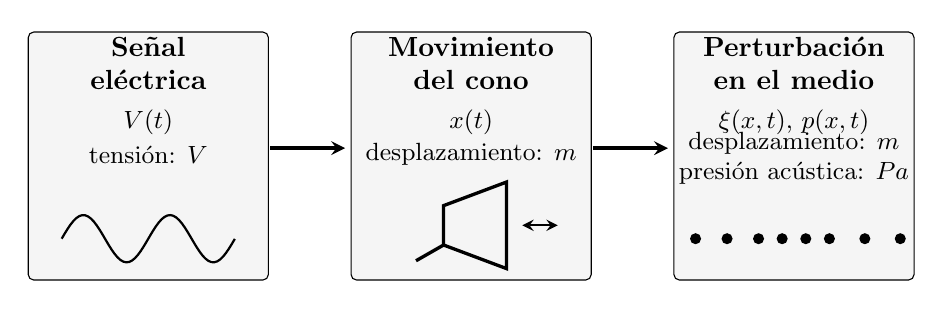
\begin{tikzpicture}[
    font=\small,
    >=stealth,
    etapa/.style={
        draw,
        rounded corners=2pt,
        minimum width=3.05cm,
        minimum height=3.15cm,
        align=center,
        fill=black!4
    }
]
    \node[etapa] (electrica) at (1.60,0) {};
    \node[etapa] (cono) at (5.70,0) {};
    \node[etapa] (medio) at (9.80,0) {};

    \node[font=\bfseries,align=center] at (1.60,1.18)
        {Señal\\eléctrica};
    \node at (1.60,0.43) {\(V(t)\)};
    \node at (1.60,0.02) {tensión: \(\text{V}\)};

    \node[font=\bfseries,align=center] at (5.70,1.18)
        {Movimiento\\del cono};
    \node at (5.70,0.43) {\(x(t)\)};
    \node at (5.70,0.02) {desplazamiento: \(\text{m}\)};

    \node[font=\bfseries,align=center] at (9.80,1.18)
        {Perturbación\\en el medio};
    \node at (9.80,0.43) {\(\xi(x,t)\), \(p(x,t)\)};
    \node[align=center] at (9.80,-0.03)
        {desplazamiento: \(\text{m}\)\\presión acústica: \(\text{Pa}\)};

    \draw[->,very thick] (3.15,0.10) -- (4.10,0.10);
    \draw[->,very thick] (7.25,0.10) -- (8.20,0.10);

    % Glifos conceptuales, sin escala.
    \draw[thick,samples=60,domain=0:1]
        plot ({0.50+2.20*\x},{-1.05+0.30*sin(720*\x)});
    \draw[very thick] (5.00,-1.33) -- (5.35,-1.13)
        -- (5.35,-0.63) -- (6.15,-0.33)
        -- (6.15,-1.43) -- (5.35,-1.13);
    \draw[<->,thick] (6.35,-0.88) -- (6.80,-0.88);
    \foreach \x in {8.55,8.95,9.35,9.65,9.95,10.25,10.70,11.15}{
        \fill (\x,-1.05) circle (2pt);
    }
\end{tikzpicture}

    \caption{Cadena conceptual desde la excitación eléctrica hasta la
    perturbación del medio. \(V(t)\), \(x(t)\), \(\xi(x,t)\) y \(p(x,t)\)
    representan magnitudes diferentes; el esquema no establece una conversión
    cuantitativa entre sus amplitudes. Elaboración propia.}
    \label{fig:u3-parlante-medio}
\end{figure}

\section{Onda viajera en espacio y tiempo}
\label{sec:u3-onda-viajera}

\subsection{Una variable que depende de posición y tiempo}
\label{sec:u3-onda-x-t}

Para describir una onda no basta con indicar cómo cambia una partícula con el
tiempo. También se debe expresar cómo cambia el estado del medio de un punto a
otro. Consideremos una onda armónica unidimensional que se propaga en el
sentido positivo de un eje espacial.

Sea \(x\) la coordenada espacial, medida en metros, y sea \(t\) el tiempo,
medido en segundos. Representaremos mediante \(\xi(x,t)\) el desplazamiento
local de partícula, medido en metros. Una onda viajera ideal puede escribirse:

\begin{equation}
    \xi(x,t)=\hat{\xi}
        \cos\left(\omega t-kx+\varphi_0\right),
    \label{eq:u3-onda-viajera}
\end{equation}

donde:

\begin{itemize}
    \item \(\hat{\xi}\) es la amplitud de desplazamiento de partícula, medida
    en metros (\(\text{m}\));
    \item \(\omega\) es la frecuencia angular, medida en radianes por segundo
    (\(\text{rad}/\text{s}\));
    \item \(k\) es el número de onda, medido en radianes por metro
    (\(\text{rad}/\text{m}\));
    \item \(\varphi_0\) es la fase inicial, expresada en radianes.
\end{itemize}

El signo \(-kx\) corresponde, con esta convención, a propagación hacia valores
crecientes de \(x\). El modelo supone una onda periódica en un medio uniforme
y no incluye todavía atenuación, reflexión ni geometrías de propagación más
complejas.

\subsection{Lectura temporal y lectura espacial}
\label{sec:u3-tiempo-espacio}

La ecuación~\eqref{eq:u3-onda-viajera} admite dos lecturas complementarias:

\begin{description}
    \item[\textbf{Gráfica temporal:}] se fija una posición \(x=x_0\) y se
    observa \(\xi(x_0,t)\). Informa cómo oscila una partícula o región del
    medio a lo largo del tiempo. La separación temporal entre estados
    equivalentes es el período \(T\).
    \item[\textbf{Fotografía espacial:}] se fija un instante \(t=t_0\) y se
    observa \(\xi(x,t_0)\). Informa cómo se distribuye el desplazamiento a lo
    largo del medio en ese instante. La separación espacial entre puntos
    consecutivos en el mismo estado de fase es la longitud de onda
    \(\lambda\).
\end{description}

Una gráfica temporal y una fotografía espacial pueden tener forma sinusoidal,
pero sus ejes horizontales representan magnitudes diferentes: segundos en el
primer caso y metros en el segundo. Confundirlas conduce a interpretar el
período como una distancia o la longitud de onda como un tiempo.

La figura~\ref{fig:u3-tiempo-espacio} utiliza los datos del ejemplo de la
sección~\ref{sec:u3-ejemplo-onda}. La variable vertical se normaliza mediante
\(\xi/\hat{\xi}\) para centrar la comparación en los ejes horizontales y no
atribuir una amplitud física inventada.

\begin{figure}[htbp]
    \centering
    % Propósito: mostrar que una gráfica temporal y una fotografía espacial de la
% misma onda tienen ejes horizontales y periodicidades diferentes.
% Origen: xi(x,t)=xi_hat cos(omega t-kx+phi_0), con phi_0=0,
% f=1000 Hz, c=340 m/s, T=1.0 ms y lambda=0.340 m, como en el ejemplo
% de la sección \ref{sec:u3-ejemplo-onda}.
% Curvas teóricas normalizadas; no representan datos medidos.
% Descripción accesible: dos paneles sinusoidales. El superior muestra
% desplazamiento normalizado frente al tiempo y marca un período de 1,0 ms.
% El inferior muestra el mismo desplazamiento frente a la posición y marca una
% longitud de onda de 0,340 m. En ambos, la fase inicial es cero.
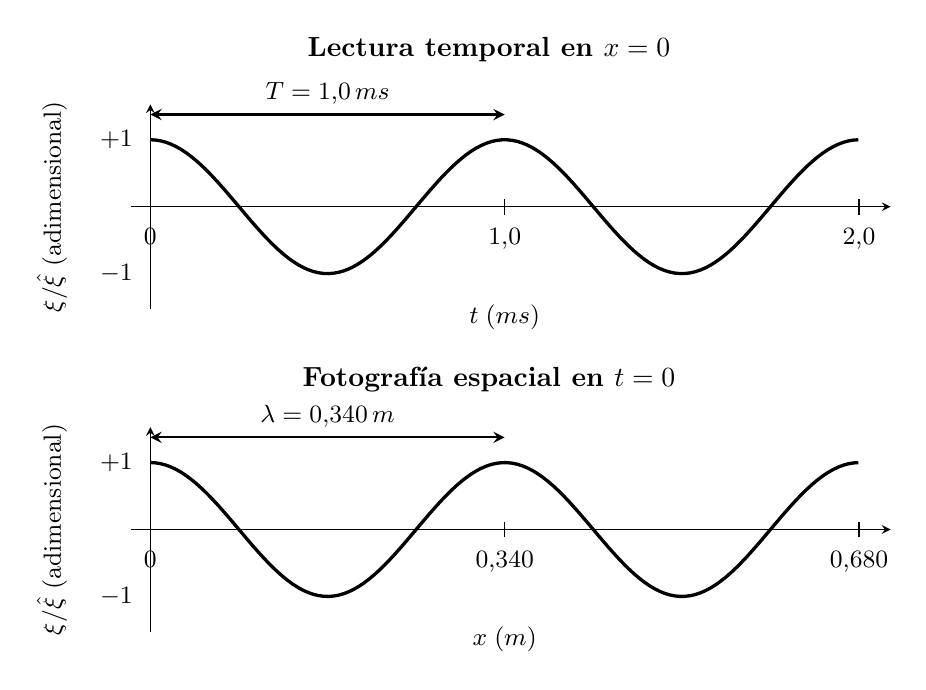
\begin{tikzpicture}[font=\small,>=stealth,x=1cm,y=1cm]
    % Panel temporal.
    \node[font=\bfseries] at (6.20,3.65)
        {Lectura temporal en \(x=0\)};
    \draw[->] (1.65,1.65) -- (11.30,1.65);
    \draw[->] (1.90,0.35) -- (1.90,2.95);
    \draw[very thick,samples=140,domain=0:2]
        plot ({1.90+4.50*\x},{1.65+0.85*cos(360*\x)});
    \node[rotate=90] at (0.65,1.65)
        {\(\xi/\hat{\xi}\) (adimensional)};
    \node at (6.40,0.25) {\(t\;(\text{ms})\)};
    \foreach \x/\lab in {0/{0},1/{1{,}0},2/{2{,}0}}{
        \pgfmathsetmacro{\xx}{1.90+4.50*\x}
        \draw (\xx,1.55) -- (\xx,1.75);
        \node[below] at (\xx,1.50) {\(\lab\)};
    }
    \node[anchor=east] at (1.80,2.50) {\(+1\)};
    \node[anchor=east] at (1.80,0.80) {\(-1\)};
    \draw[<->,thick] (1.90,2.82) -- (6.40,2.82)
        node[midway,above] {\(T=1{,}0\,\text{ms}\)};

    % Panel espacial.
    \node[font=\bfseries] at (6.20,-0.55)
        {Fotografía espacial en \(t=0\)};
    \draw[->] (1.65,-2.45) -- (11.30,-2.45);
    \draw[->] (1.90,-3.75) -- (1.90,-1.15);
    \draw[very thick,samples=140,domain=0:2]
        plot ({1.90+4.50*\x},{-2.45+0.85*cos(360*\x)});
    \node[rotate=90] at (0.65,-2.45)
        {\(\xi/\hat{\xi}\) (adimensional)};
    \node at (6.40,-3.85) {\(x\;(\text{m})\)};
    \foreach \q/\lab in {0/{0},1/{0{,}340},2/{0{,}680}}{
        \pgfmathsetmacro{\xx}{1.90+4.50*\q}
        \draw (\xx,-2.55) -- (\xx,-2.35);
        \node[below] at (\xx,-2.60) {\(\lab\)};
    }
    \node[anchor=east] at (1.80,-1.60) {\(+1\)};
    \node[anchor=east] at (1.80,-3.30) {\(-1\)};
    \draw[<->,thick] (1.90,-1.28) -- (6.40,-1.28)
        node[midway,above] {\(\lambda=0{,}340\,\text{m}\)};
\end{tikzpicture}

    \caption{Dos lecturas de la misma onda ideal con
    \(f=1000\,\text{Hz}\), \(c=340\,\text{m}/\text{s}\) y
    \(\varphi_0=0\). Al fijar la posición se mide
    \(T=1{,}0\,\text{ms}\); al fijar el instante se mide
    \(\lambda=0{,}340\,\text{m}\). Son curvas teóricas normalizadas,
    elaboradas a partir de la ecuación~\eqref{eq:u3-onda-viajera}.}
    \label{fig:u3-tiempo-espacio}
\end{figure}

\subsection{Longitud de onda y velocidad de propagación}
\label{sec:u3-longitud-velocidad}

El número de onda y la longitud de onda se relacionan mediante:

\begin{equation}
    k=\frac{2\pi}{\lambda},
    \label{eq:u3-numero-onda}
\end{equation}

donde \(\lambda\) se mide en metros. Durante un período, un estado de fase de
la onda avanza una longitud de onda. Por lo tanto, la velocidad de propagación
\(c\), medida en metros por segundo, satisface:

\begin{equation}
    c=\frac{\lambda}{T}=\lambda f=\frac{\omega}{k}.
    \label{eq:u3-velocidad-onda}
\end{equation}

En un medio uniforme, si la fuente mantiene fija la frecuencia y cambia la
velocidad de propagación, también cambia la longitud de onda:

\begin{equation}
    \lambda=\frac{c}{f}.
    \label{eq:u3-longitud-onda}
\end{equation}

Este cambio de \(\lambda\) no implica por sí solo un cambio de frecuencia ni
de altura tonal. La velocidad depende de las propiedades del medio, como se
introdujo en la Unidad~\ref{chap:unidad-2}; aquí interesa su relación
cinemática con \(f\) y \(\lambda\).

\subsection{Ejemplo resuelto: lectura temporal y espacial}
\label{sec:u3-ejemplo-onda}

Para un modelo en aire se adopta una velocidad constante
\(c=340\,\text{m}/\text{s}\) y una frecuencia \(f=1000\,\text{Hz}\). Estos
valores se usan como datos del problema, no como valores universales.

El período es:

\[
    T=\frac{1}{1000\,\text{s}^{-1}}
      =1{,}0\times10^{-3}\,\text{s}
      =1{,}0\,\text{ms}.
\]

La frecuencia angular es:

\[
    \omega=2\pi f
      =2\pi(1000\,\text{s}^{-1})
      \approx6{,}28\times10^{3}\,\text{rad}/\text{s}.
\]

La longitud de onda y el número de onda son:

\[
    \lambda=\frac{340\,\text{m}/\text{s}}
                   {1000\,\text{s}^{-1}}
            =0{,}340\,\text{m},
\]

\[
    k=\frac{2\pi}{0{,}340\,\text{m}}
      \approx18{,}5\,\text{rad}/\text{m}.
\]

En una gráfica temporal tomada en un punto fijo se separan
\(1{,}0\,\text{ms}\) dos máximos consecutivos. En una fotografía espacial
tomada en un instante fijo se separan \(0{,}340\,\text{m}\). Se trata de la
misma periodicidad expresada en dominios distintos.

\subsection{Velocidad de partícula y velocidad de propagación}
\label{sec:u3-velocidades}

La \textbf{velocidad de partícula} describe el movimiento local de una pequeña
región del medio. Se representará mediante \(u(x,t)\) y se medirá en metros por
segundo. Para el desplazamiento de la ecuación~\eqref{eq:u3-onda-viajera}:

\begin{equation}
    u(x,t)=-\omega\hat{\xi}
        \sin\left(\omega t-kx+\varphi_0\right).
    \label{eq:u3-velocidad-particula}
\end{equation}

Su valor absoluto máximo es:

\begin{equation}
    u_{\max}=\omega\hat{\xi}.
    \label{eq:u3-velocidad-particula-max}
\end{equation}

La \textbf{velocidad de propagación} \(c\), en cambio, describe el avance de un
estado de fase de la onda. Aunque \(u\) y \(c\) se expresan en
\(\text{m}/\text{s}\), no representan la misma magnitud:

\begin{itemize}
    \item \(u(x,t)\) cambia con la posición y el tiempo y puede invertir su
    sentido durante cada ciclo;
    \item \(c\) caracteriza la propagación en el medio dentro del modelo
    adoptado;
    \item una partícula no debe recorrer una longitud de onda para que la
    perturbación avance esa distancia.
\end{itemize}

Por ejemplo, si en el modelo anterior se adopta
\(\hat{\xi}=2{,}0\,\mu\text{m}=2{,}0\times10^{-6}\,\text{m}\), la velocidad
local máxima es:

\[
    u_{\max}
      =(6{,}28\times10^{3}\,\text{s}^{-1})
       (2{,}0\times10^{-6}\,\text{m})
      \approx1{,}26\times10^{-2}\,\text{m}/\text{s}.
\]

Este valor no debe confundirse con
\(c=340\,\text{m}/\text{s}\). La amplitud de desplazamiento se eligió como
dato hipotético para comparar las dos definiciones y no describe una
medición clínica.

\section{Fase, superposición e interferencia}
\label{sec:u3-superposicion}

\subsection{Fase inicial y diferencia de fase}
\label{sec:u3-diferencia-fase}

La fase inicial \(\varphi_0\) indica el estado de una oscilación cuando
\(t=0\). Para comparar dos oscilaciones interesa la
\textbf{diferencia de fase}. Si sus fases iniciales son
\(\varphi_1\) y \(\varphi_2\), se define:

\begin{equation}
    \Delta\varphi=\varphi_2-\varphi_1,
    \label{eq:u3-diferencia-fase}
\end{equation}

y se expresa en radianes. Dos señales pueden tener fases iniciales diferentes
pero una diferencia de fase constante si comparten la misma frecuencia.

\subsection{Principio de superposición}
\label{sec:u3-principio-superposicion}

En un sistema lineal, cuando dos perturbaciones coinciden en una misma
posición y un mismo instante, la perturbación resultante es la suma algebraica
de ambas:

\begin{equation}
    y_\mathrm{R}(x,t)=y_1(x,t)+y_2(x,t).
    \label{eq:u3-superposicion}
\end{equation}

Las variables \(y_1\), \(y_2\) e \(y_\mathrm{R}\) deben representar la misma
magnitud y tener la misma unidad. El principio no autoriza, por ejemplo, a
sumar directamente un desplazamiento en metros con una presión en pascales.

Para dos oscilaciones de igual frecuencia e igual amplitud \(A\), evaluadas en
un mismo punto:

\[
    y_1(t)=A\cos(\omega t),
    \qquad
    y_2(t)=A\cos(\omega t+\Delta\varphi),
\]

la amplitud de la resultante es:

\begin{equation}
    A_\mathrm{R}
      =2A\left|\cos\left(\frac{\Delta\varphi}{2}\right)\right|.
    \label{eq:u3-amplitud-resultante}
\end{equation}

Se distinguen tres situaciones:

\begin{description}
    \item[\textbf{Interferencia constructiva:}]
    si \(\Delta\varphi=0\), los máximos coinciden y
    \(A_\mathrm{R}=2A\).
    \item[\textbf{Interferencia parcial:}]
    para otros desfases, la amplitud resultante toma un valor intermedio.
    Por ejemplo, si \(\Delta\varphi=\pi/2\,\text{rad}\),
    \(A_\mathrm{R}=\sqrt{2}A\).
    \item[\textbf{Interferencia destructiva total:}]
    si \(\Delta\varphi=\pi\,\text{rad}\), las señales se cancelan solo cuando
    también poseen igual amplitud y se comparan en el mismo punto.
\end{description}

Si las amplitudes son diferentes, un desfase de \(\pi\,\text{rad}\) produce
una reducción, pero no una cancelación total. Si las frecuencias son
diferentes, la diferencia de fase varía con el tiempo y la resultante también
puede cambiar de amplitud.

La figura~\ref{fig:u3-superposicion-desfase} compara los tres casos mediante
señales normalizadas. Las líneas representan una misma magnitud adimensional;
no se las interpreta como presión, desplazamiento o tensión sin una
calibración adicional.

\begin{figure}[htbp]
    \centering
    % Propósito: comparar la suma de dos sinusoides de igual frecuencia y amplitud
% para tres diferencias de fase.
% Origen: y_1=cos(omega t), y_2=cos(omega t+Delta phi) y
% y_R=y_1+y_2, ecuaciones \eqref{eq:u3-superposicion} y
% \eqref{eq:u3-amplitud-resultante}.
% Curvas teóricas normalizadas; no representan datos medidos.
% Descripción accesible: tres paneles muestran dos señales y su suma. Con
% diferencia de fase cero, la suma duplica la amplitud; con pi sobre dos, la
% amplitud es raíz de dos; con pi, la suma es cero en todo instante.
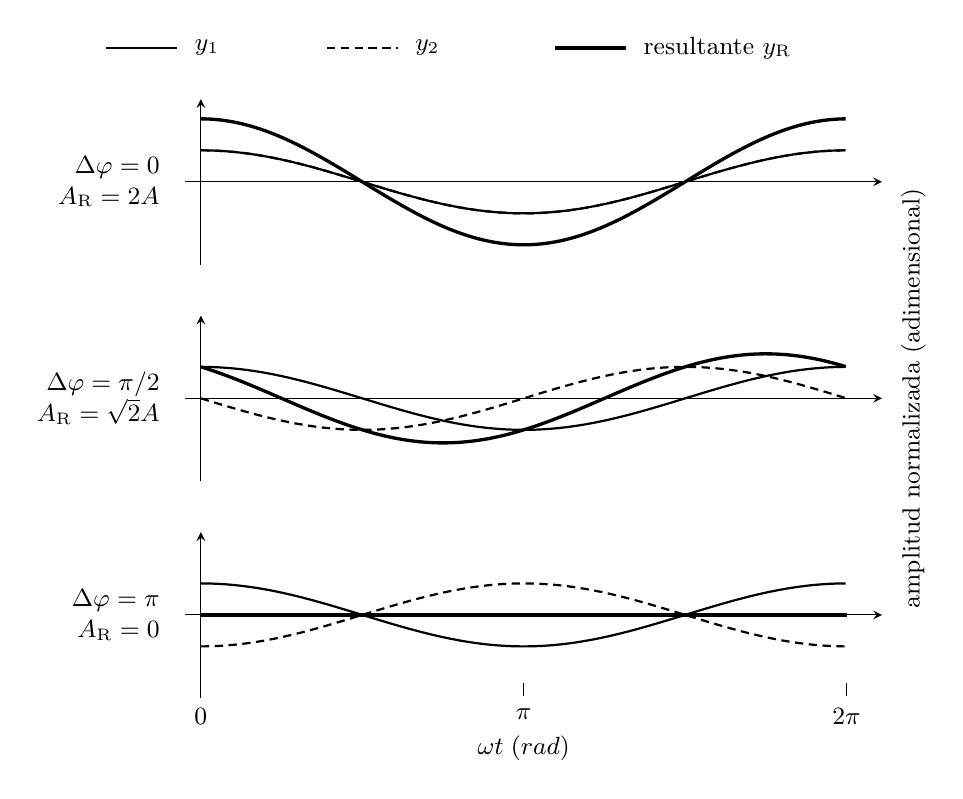
\begin{tikzpicture}[font=\small,>=stealth,x=1cm,y=1cm]
    % Leyenda.
    \draw[thick] (1.30,4.45) -- (2.20,4.45);
    \node[anchor=west] at (2.30,4.45) {\(y_1\)};
    \draw[thick,densely dashed] (4.10,4.45) -- (5.00,4.45);
    \node[anchor=west] at (5.10,4.45) {\(y_2\)};
    \draw[very thick] (7.00,4.45) -- (7.90,4.45);
    \node[anchor=west] at (8.00,4.45) {resultante \(y_\mathrm{R}\)};

    % Ejes comunes.
    \foreach \yy/\fase/\amp in {2.75/{0}/{2A},0/{\pi/2}/{\sqrt{2}A},-2.75/{\pi}/{0}}{
        \draw[->] (2.30,\yy) -- (11.15,\yy);
        \draw[->] (2.50,\yy-1.05) -- (2.50,\yy+1.05);
        \node[anchor=east,align=right] at (2.10,\yy)
            {\(\Delta\varphi=\fase\)\\\(A_\mathrm{R}=\amp\)};
    }

    % Caso Delta phi = 0.
    \draw[thick,samples=120,domain=0:1]
        plot ({2.50+8.20*\x},{2.75+0.40*cos(360*\x)});
    \draw[thick,densely dashed,samples=120,domain=0:1]
        plot ({2.50+8.20*\x},{2.75+0.40*cos(360*\x)});
    \draw[very thick,samples=120,domain=0:1]
        plot ({2.50+8.20*\x},{2.75+0.80*cos(360*\x)});

    % Caso Delta phi = pi/2.
    \draw[thick,samples=120,domain=0:1]
        plot ({2.50+8.20*\x},{0.40*cos(360*\x)});
    \draw[thick,densely dashed,samples=120,domain=0:1]
        plot ({2.50+8.20*\x},{0.40*cos(360*\x+90)});
    \draw[very thick,samples=120,domain=0:1]
        plot ({2.50+8.20*\x},{0.40*(cos(360*\x)+cos(360*\x+90))});

    % Caso Delta phi = pi.
    \draw[thick,samples=120,domain=0:1]
        plot ({2.50+8.20*\x},{-2.75+0.40*cos(360*\x)});
    \draw[thick,densely dashed,samples=120,domain=0:1]
        plot ({2.50+8.20*\x},{-2.75+0.40*cos(360*\x+180)});
    \draw[very thick] (2.50,-2.75) -- (10.70,-2.75);

    % Etiquetas del eje de fase.
    \foreach \q/\lab in {0/{0},0.5/{\pi},1/{2\pi}}{
        \pgfmathsetmacro{\xx}{2.50+8.20*\q}
        \draw (\xx,-3.78) -- (\xx,-3.62);
        \node[below] at (\xx,-3.82) {\(\lab\)};
    }
    \node at (6.60,-4.45) {\(\omega t\;(\text{rad})\)};
    \node[rotate=90] at (11.55,0)
        {amplitud normalizada (adimensional)};
\end{tikzpicture}

    \caption{Superposición de dos sinusoides con igual frecuencia e igual
    amplitud \(A\). La resultante tiene amplitud \(2A\),
    \(\sqrt{2}A\) o cero para diferencias de fase \(0\),
    \(\pi/2\) y \(\pi\), respectivamente. La cancelación total del último
    panel depende también de las condiciones indicadas en el texto.
    Elaboración propia a partir de la
    ecuación~\eqref{eq:u3-amplitud-resultante}.}
    \label{fig:u3-superposicion-desfase}
\end{figure}

\subsection{Alcance del ejemplo de cancelación activa}
\label{sec:u3-anc}

La cancelación activa de ruido utiliza medición, procesamiento y una
señal de control para reducir determinadas componentes del campo sonoro en una
región de interés. Su funcionamiento no equivale a crear una ``onda opuesta''
que elimine todo el ruido en cualquier punto; el resultado depende, entre
otros factores, de la frecuencia, la geometría, los retardos y la posición del
receptor~\cite{moser2009}. Este ejemplo permite aplicar la superposición, pero no demuestra
por sí solo una mejora de la inteligibilidad ni reemplaza el estudio técnico
de un dispositivo.

\section{Relación con Fonoaudiología}
\label{sec:u3-fonoaudiologia}

Los modelos de esta unidad aportan distinciones necesarias para interpretar
situaciones posteriores:

\begin{description}
    \item[\textbf{Producción y recepción del sonido:}]
    una fuente puede oscilar localmente mientras la perturbación se propaga
    por el medio hasta el receptor.
    \item[\textbf{Registros temporales:}]
    una forma de onda permite medir período, frecuencia y fase si se conocen
    los ejes. Su amplitud solo adquiere una unidad física cuando el sistema de
    medición está definido y calibrado.
    \item[\textbf{Tonos audiométricos:}]
    la audiometría liminar utiliza estímulos y niveles calibrados,
    procedimientos de presentación y respuestas repetidas para estimar
    umbrales. Una respuesta aislada ante un tono no permite concluir por sí
    sola que existe o no una pérdida auditiva~\cite{ashaPureTone2005,iso8253_1_2010}.
    \item[\textbf{Magnitud física y atributo perceptual:}]
    la frecuencia del estímulo se mide en hertz; la altura tonal o
    \emph{pitch} es un atributo perceptual. De manera análoga, una amplitud
    física no es un sinónimo de sonoridad.
\end{description}

La presión acústica, los niveles en decibeles, los valores pico y eficaz y la
impedancia se desarrollarán en la Unidad~\ref{chap:unidad-4}. La
interpretación clínica de una evaluación se reservará para la unidad
correspondiente.

\section{Errores frecuentes}
\label{sec:u3-errores}

\begin{description}[style=nextline]
    \item[\textbf{La partícula viaja con la onda.}]
    La partícula oscila localmente; la perturbación se propaga mediante la
    interacción entre regiones vecinas.
    \item[\textbf{Velocidad de partícula y velocidad de propagación son la
    misma magnitud.}]
    Ambas se miden en \(\text{m}/\text{s}\), pero describen movimientos
    diferentes.
    \item[\textbf{Toda sinusoide dibujada es una onda espacial.}]
    Una sinusoide puede representar una oscilación temporal, una fotografía
    espacial o una magnitud eléctrica. Los ejes determinan la interpretación.
    \item[\textbf{La amplitud es el volumen.}]
    La amplitud debe asociarse con una magnitud y una unidad. ``Volumen'' no
    nombra una magnitud acústica.
    \item[\textbf{La frecuencia es el \emph{pitch}.}]
    La frecuencia es una magnitud física; el \emph{pitch} es un atributo
    perceptual.
    \item[\textbf{La fase inicial y la diferencia de fase son
    intercambiables.}]
    La fase inicial describe una señal respecto del origen temporal; la
    diferencia de fase compara dos señales.
    \item[\textbf{Un desfase de \(\pi\) siempre elimina dos ondas.}]
    La cancelación total también requiere igual frecuencia, igual amplitud y
    comparación en el mismo punto.
    \item[\textbf{Una frecuencia alta se propaga necesariamente más rápido.}]
    En el modelo \(c=\lambda f\), la velocidad está determinada por el medio;
    al cambiar \(f\) puede cambiar \(\lambda\) sin que cambie \(c\).
\end{description}

\section{Síntesis}
\label{sec:u3-sintesis}

Una oscilación describe el movimiento local de un sistema alrededor de una
posición de equilibrio. Una onda describe la propagación de una perturbación
a través de un medio. En una onda mecánica, las partículas pueden oscilar
localmente mientras el estado de perturbación y la energía asociada avanzan.

El movimiento armónico simple es un modelo ideal en el que la aceleración es
proporcional al desplazamiento y apunta hacia el equilibrio. La amplitud
describe el máximo desplazamiento; la frecuencia, el período y la frecuencia
angular describen la repetición temporal; la fase inicial ubica el sistema
dentro del ciclo. Posición, velocidad y aceleración tienen la misma
frecuencia, pero alcanzan sus máximos en instantes diferentes.

Una onda viajera depende de posición y tiempo. El período se reconoce en una
gráfica temporal y la longitud de onda en una fotografía espacial. Las
relaciones \(T=1/f\), \(\omega=2\pi f\), \(k=2\pi/\lambda\) y
\(c=\lambda f=\omega/k\) conectan ambas representaciones. La velocidad local
de partícula no debe confundirse con la velocidad de propagación.

La superposición suma perturbaciones de la misma magnitud. La diferencia de
fase determina si la combinación es constructiva, parcial o destructiva; la
cancelación total es un caso ideal con condiciones adicionales. Estas
distinciones preparan el estudio de las magnitudes acústicas de la
Unidad~\ref{chap:unidad-4}.

\section{Ejercicios de autoevaluación}
\label{sec:u3-ejercicios}

La secuencia comienza con distinciones conceptuales y lectura de figuras,
continúa con cálculos guiados y autónomos, y termina con aplicaciones,
integración y análisis de distractores. En los ejercicios numéricos se debe
escribir la ecuación utilizada, conservar las unidades durante el cálculo,
redondear solo el resultado final e interpretar su significado físico.

\subsection*{Preguntas conceptuales}

\begin{enumerate}[label=\textbf{C\arabic*.},leftmargin=*]
    \item Una región comprimida avanza por un resorte mientras una espira
    marcada se desplaza alrededor de su posición inicial. Identifique cuál
    observación corresponde al movimiento local y cuál a la propagación.

    \item Compare una onda longitudinal y una transversal indicando la
    dirección del movimiento local respecto de la dirección de propagación.

    \item En un MAS, compare posición, velocidad y aceleración cuando el
    sistema se encuentra en un extremo y cuando pasa por el equilibrio.

    \item Explique por qué una gráfica sinusoidal sin nombres ni unidades en
    sus ejes no puede interpretarse automáticamente como presión acústica,
    desplazamiento ni sonoridad.

    \item Distinga fase inicial y diferencia de fase mediante un ejemplo con
    dos oscilaciones.

    \item Explique por qué \(u=0{,}020\,\text{m}/\text{s}\) y
    \(c=340\,\text{m}/\text{s}\) pueden corresponder a una misma onda sin
    constituir una contradicción.

    \item Distinga frecuencia física y \emph{pitch}. Distinga además amplitud
    de desplazamiento y amplitud de presión acústica.

    \item Indique qué condiciones adicionales se requieren para que dos
    sinusoides con \(\Delta\varphi=\pi\,\text{rad}\) se cancelen totalmente.
\end{enumerate}

\subsection*{Identificación e interpretación de gráficos}

\begin{enumerate}[label=\textbf{R\arabic*.},leftmargin=*]
    \item Observe la figura~\ref{fig:u3-oscilacion-propagacion}.
    \begin{enumerate}[label=\alph*)]
        \item Identifique qué flecha representa el movimiento local y cuál
        representa la propagación.
        \item Explique por qué la región marcada no debe recorrer la misma
        distancia que la compresión.
    \end{enumerate}

    \item Utilice la figura~\ref{fig:u3-mas-cinematica}.
    \begin{enumerate}[label=\alph*)]
        \item Lea los valores normalizados de posición, velocidad y
        aceleración en \(t/T=1/4\) y en \(t/T=1/2\).
        \item Indique en cuál de esos instantes el sistema pasa por el
        equilibrio y en cuál se encuentra en un extremo.
        \item Explique por qué las ordenadas normalizadas no se expresan en
        metros, metros por segundo o metros por segundo cuadrado.
    \end{enumerate}

    \item En la figura~\ref{fig:u3-tiempo-espacio}:
    \begin{enumerate}[label=\alph*)]
        \item identifique qué variable se mantiene fija en cada panel;
        \item lea el período \(T\) y la longitud de onda \(\lambda\);
        \item calcule \(f\) y \(c\) a partir de esas lecturas;
        \item explique por qué \(1{,}0\,\text{ms}\) y
        \(0{,}340\,\text{m}\) describen periodicidades diferentes de la misma
        onda.
    \end{enumerate}

    \item Compare los tres paneles de la
    figura~\ref{fig:u3-superposicion-desfase}.
    \begin{enumerate}[label=\alph*)]
        \item Asocie cada panel con
        \(\Delta\varphi=0\), \(\pi/2\,\text{rad}\) o
        \(\pi\,\text{rad}\).
        \item Ordene las amplitudes resultantes de mayor a menor.
        \item Explique por qué solo pueden sumarse las ordenadas si todas
        representan la misma magnitud.
    \end{enumerate}

    \item Observe la figura~\ref{fig:u3-parlante-medio}.
    \begin{enumerate}[label=\alph*)]
        \item Identifique la magnitud y la unidad indicadas en cada etapa.
        \item Explique qué información adicional se necesitaría para convertir
        una señal eléctrica o digital en presión acústica expresada en
        pascales.
    \end{enumerate}
\end{enumerate}

\subsection*{Ejercicios numéricos guiados}

\begin{enumerate}[label=\textbf{G\arabic*.},leftmargin=*]
    \item Una oscilación tiene frecuencia \(f=250\,\text{Hz}\). Utilice
    \(T=1/f\) y \(\omega=2\pi f\).
    \begin{enumerate}[label=\alph*)]
        \item Calcule el período \(T\) en segundos y milisegundos.
        \item Calcule la frecuencia angular \(\omega\).
        \item Determine cuántos ciclos ocurren en \(20\,\text{ms}\).
    \end{enumerate}

    \item Un sistema realiza un MAS con
    \(A=2{,}0\,\text{mm}\), \(f=5{,}0\,\text{Hz}\) y
    \(\varphi_0=0\,\text{rad}\).
    \begin{enumerate}[label=\alph*)]
        \item Convierta la amplitud a metros y calcule \(\omega\).
        \item Escriba \(x(t)\) con los valores en unidades SI.
        \item Calcule \(x(0)\), \(v(0)\) y \(a(0)\).
        \item Indique hacia dónde apunta la aceleración en ese instante.
    \end{enumerate}

    \item En un medio uniforme se adopta
    \(c=340\,\text{m}/\text{s}\) para una onda de
    \(f=2000\,\text{Hz}\). Utilice
    \(\lambda=c/f\), \(k=2\pi/\lambda\) y la definición de velocidad.
    \begin{enumerate}[label=\alph*)]
        \item Calcule \(\lambda\).
        \item Calcule \(k\).
        \item Calcule el tiempo que tarda un estado de fase en avanzar
        \(0{,}85\,\text{m}\).
        \item Indique qué magnitud cambiaría si \(f\) aumentara y \(c\)
        permaneciera constante.
    \end{enumerate}

    \item Dos desplazamientos de igual frecuencia y amplitud
    \(A=3{,}0\,\text{mm}\), evaluados en el mismo punto, tienen
    \(\Delta\varphi=\pi/2\,\text{rad}\). Utilice
    \(A_\mathrm{R}=2A|\cos(\Delta\varphi/2)|\).
    \begin{enumerate}[label=\alph*)]
        \item Calcule la amplitud resultante.
        \item Compare el resultado con los casos
        \(\Delta\varphi=0\,\text{rad}\) y
        \(\Delta\varphi=\pi\,\text{rad}\).
    \end{enumerate}
\end{enumerate}

\subsection*{Ejercicios numéricos autónomos}

\begin{enumerate}[label=\textbf{N\arabic*.},leftmargin=*]
    \item Un oscilador masa--resorte ideal tiene
    \(m=2{,}0\times10^{-2}\,\text{kg}\) y
    \(k=50\,\text{N}/\text{m}\). Calcule \(\omega\), \(f\) y \(T\).

    \item Un MAS tiene \(A=0{,}20\,\text{mm}\),
    \(f=120\,\text{Hz}\) y
    \(\varphi_0=\pi/2\,\text{rad}\). Calcule \(x(0)\), \(v(0)\) y
    \(a(0)\), con unidades SI, e interprete el sentido inicial del
    movimiento.

    \item En una gráfica temporal, dos máximos consecutivos están separados
    por \(0{,}50\,\text{ms}\). Para el medio se adopta
    \(c=344\,\text{m}/\text{s}\). Calcule \(T\), \(f\), \(\lambda\) y \(k\).

    \item Una onda presenta
    \(\hat{\xi}=4{,}0\,\mu\text{m}\) y
    \(f=500\,\text{Hz}\). Calcule \(u_{\max}\). Si se adopta
    \(c=343\,\text{m}/\text{s}\), calcule además \(c/u_{\max}\) y explique
    por qué esa razón no significa que una partícula quede retrasada respecto
    de una ``partícula que viaja'' con la onda.

    \item En el mismo punto del medio se superponen:
    \[
        y_1(t)=(5{,}0\,\mu\text{m})
        \cos\left[2\pi(300\,\text{s}^{-1})t\right],
    \]
    \[
        y_2(t)=(3{,}0\,\mu\text{m})
        \cos\left[2\pi(300\,\text{s}^{-1})t+\pi\,\text{rad}\right].
    \]
    Obtenga \(y_\mathrm{R}(t)\), indique su amplitud y explique por qué no hay
    cancelación total.
\end{enumerate}

\subsection*{Aplicaciones en Fonoaudiología}

\begin{enumerate}[label=\textbf{F\arabic*.},leftmargin=*]
    \item En una actividad de percepción se presentan dos tonos puros
    idealizados con \(f_1=500\,\text{Hz}\) y
    \(f_2=1000\,\text{Hz}\). Una persona informa que el segundo tiene mayor
    \emph{pitch}.
    \begin{enumerate}[label=\alph*)]
        \item Calcule \(T_1\) y \(T_2\).
        \item Separe los datos físicos de la respuesta perceptual.
        \item Explique por qué el informe perceptual no cambia los valores de
        frecuencia medidos.
    \end{enumerate}

    \item Para un modelo ideal del cono de un parlante se registra:
    \[
        x(t)=(0{,}030\,\text{mm})
        \cos\left[2\pi(400\,\text{s}^{-1})t\right].
    \]
    \begin{enumerate}[label=\alph*)]
        \item Identifique la amplitud de desplazamiento y la frecuencia.
        \item Calcule \(T\) y \(v_{\max}\).
        \item Explique por qué esos resultados no determinan la amplitud de
        presión acústica ni la sonoridad.
    \end{enumerate}

    \newpage
    \item Un micrófono calibrado registra en un punto:
    \[
        p(t)=(0{,}020\,\text{Pa})
        \cos\left[2\pi(1000\,\text{s}^{-1})t\right].
    \]
    \begin{enumerate}[label=\alph*)]
        \item Identifique la amplitud de presión, la frecuencia y el período.
        \item Indique qué información no permite obtener esta ecuación acerca
        del desplazamiento de partícula.
        \item Explique por qué la amplitud de presión no es una medida directa
        de sonoridad.
    \end{enumerate}
\end{enumerate}

\subsection*{Pregunta integradora}

\begin{enumerate}[label=\textbf{I\arabic*.},leftmargin=*]
    \item Se propone un modelo ideal, no clínico, de una cadena
    parlante--aire. El cono oscila con amplitud
    \(A=0{,}050\,\text{mm}\), frecuencia
    \(f=800\,\text{Hz}\) y fase inicial
    \(\varphi_0=0\,\text{rad}\). En el aire se adopta
    \(c=344\,\text{m}/\text{s}\) y una amplitud local de desplazamiento de
    partícula \(\hat{\xi}=2{,}0\,\mu\text{m}\). En un punto llega además una
    segunda perturbación de la misma magnitud, frecuencia y amplitud, con
    \(\Delta\varphi=\pi/2\,\text{rad}\).
    \begin{enumerate}[label=\alph*)]
        \item Distinga la oscilación del cono, el movimiento local de las
        partículas y la propagación de la onda.
        \item Calcule \(T\) y \(\omega\).
        \item Calcule la rapidez máxima del cono.
        \item Calcule \(\lambda\) y \(k\).
        \item Calcule \(u_{\max}\) para las partículas del aire y compárelo
        con \(c\).
        \item Calcule la amplitud resultante del desplazamiento local en el
        punto donde coinciden ambas perturbaciones.
        \item Indique qué datos adicionales serían necesarios para determinar
        presión acústica y por qué los resultados no predicen por sí solos una
        respuesta perceptual o clínica.
    \end{enumerate}
\end{enumerate}

\subsection*{Errores frecuentes y distractores}

En cada caso, determine si la respuesta propuesta es correcta. Si no lo es,
identifique el distractor y escriba la corrección.

\begin{enumerate}[label=\textbf{D\arabic*.},leftmargin=*]
    \item Para \(f=1000\,\text{Hz}\), se propone
    \(T=1000\,\text{s}\) porque período y frecuencia tienen el mismo valor
    numérico.

    \item En una gráfica cuyo eje horizontal es \(t\) en milisegundos y cuyo
    eje vertical es \(\xi\) en micrómetros, se propone medir la distancia entre
    máximos para obtener \(\lambda\).

    \item Cuando un MAS se encuentra en \(x=+A\), se propone que la velocidad
    y la aceleración son máximas y apuntan en el sentido positivo.

    \item Como \(u\) y \(c\) se expresan en
    \(\text{m}/\text{s}\), se propone que ambas representan la velocidad con
    la que el sonido recorre el medio.

    \item Dos sinusoides tienen
    \(\Delta\varphi=\pi\,\text{rad}\). Se propone que siempre se cancelan,
    aunque sus amplitudes sean diferentes.

    \item En un mismo medio, una fuente duplica su frecuencia. Se propone que
    la velocidad de propagación también se duplica y que \(\lambda\)
    permanece constante.

    \item Se propone que una amplitud de desplazamiento de
    \(3{,}0\,\mu\text{m}\) equivale a una amplitud de presión de
    \(3{,}0\,\text{Pa}\) y determina una sonoridad única.
\end{enumerate}

\section{Soluciones de los ejercicios}
\label{sec:u3-soluciones}

\subsection*{Preguntas conceptuales}

\begin{enumerate}[label=\textbf{C\arabic*.},leftmargin=*]
    \item El desplazamiento de la espira es movimiento local. El avance de la
    región comprimida es propagación de la perturbación.

    \item En una onda longitudinal, el movimiento local es paralelo a la
    propagación; en una transversal, es perpendicular.

    \item En un extremo, \(x=\pm A\), \(v=0\) y la aceleración tiene valor
    absoluto máximo y apunta hacia el equilibrio. Al pasar por el equilibrio,
    \(x=0\), la rapidez es máxima y \(a=0\).

    \item La forma sinusoidal solo informa una dependencia matemática. Los
    ejes deben identificar la variable y su unidad para distinguir, por
    ejemplo, metros, pascales o una señal adimensional. La sonoridad es un
    atributo perceptual, no una lectura directa de la curva.

    \item La fase inicial ubica una oscilación respecto de \(t=0\). La
    diferencia de fase compara dos oscilaciones; por ejemplo, si
    \(\varphi_1=0\) y \(\varphi_2=\pi/2\,\text{rad}\), entonces
    \(\Delta\varphi=\pi/2\,\text{rad}\).

    \item \(u\) describe la velocidad local de partícula y cambia durante el
    ciclo; \(c\) describe el avance de la perturbación. Comparten unidad, pero
    no significado físico.

    \item La frecuencia se mide en hertz y caracteriza la repetición temporal
    del estímulo; el \emph{pitch} es un atributo perceptual. Una amplitud de
    desplazamiento se mide en metros y una amplitud de presión acústica en
    pascales. Ninguna de ellas es, por sí sola, una medida de sonoridad.

    \item Además del desfase de \(\pi\,\text{rad}\), se requieren igual
    frecuencia, igual amplitud y comparación en el mismo punto.
\end{enumerate}

\subsection*{Identificación e interpretación de gráficos}

\begin{enumerate}[label=\textbf{R\arabic*.},leftmargin=*]
    \item
    \begin{enumerate}[label=\alph*)]
        \item Las flechas cortas asociadas con la región marcada representan
        el movimiento local. La flecha larga representa el avance de la
        compresión con velocidad de propagación \(c\).
        \item La región marcada oscila alrededor de su equilibrio; la
        compresión es un estado de perturbación que se transmite entre
        regiones vecinas. Por eso sus recorridos no coinciden.
    \end{enumerate}

    \item
    \begin{enumerate}[label=\alph*)]
        \item En \(t/T=1/4\):
        \[
            x/A=0,\qquad v/(\omega A)=-1,\qquad
            a/(\omega^{2}A)=0.
        \]
        En \(t/T=1/2\):
        \[
            x/A=-1,\qquad v/(\omega A)=0,\qquad
            a/(\omega^{2}A)=+1.
        \]
        \item En \(t/T=1/4\) el sistema pasa por el equilibrio hacia valores
        negativos. En \(t/T=1/2\) se encuentra en el extremo negativo.
        \item Cada ordenada es el cociente entre una magnitud y su valor de
        escala con la misma unidad; por eso el resultado es adimensional.
    \end{enumerate}

    \item
    \begin{enumerate}[label=\alph*)]
        \item En el panel temporal se fija \(x=0\); en el espacial se fija
        \(t=0\).
        \item Se leen \(T=1{,}0\,\text{ms}\) y
        \(\lambda=0{,}340\,\text{m}\).
        \item
        \[
            f=\frac{1}{1{,}0\times10^{-3}\,\text{s}}
              =1000\,\text{Hz},
        \]
        \[
            c=\lambda f
              =(0{,}340\,\text{m})(1000\,\text{s}^{-1})
              =340\,\text{m}/\text{s}.
        \]
        \item El período es una separación temporal entre estados
        equivalentes en un punto fijo; la longitud de onda es una separación
        espacial entre puntos equivalentes en un instante fijo.
    \end{enumerate}

    \item
    \begin{enumerate}[label=\alph*)]
        \item Los paneles corresponden, respectivamente, a
        \(\Delta\varphi=0\), \(\pi/2\,\text{rad}\) y
        \(\pi\,\text{rad}\).
        \item Las amplitudes resultantes son
        \(2A>\sqrt{2}A>0\).
        \item La suma algebraica exige que las ordenadas representen la misma
        magnitud y tengan la misma unidad.
    \end{enumerate}

    \item
    \begin{enumerate}[label=\alph*)]
        \item \(V(t)\) es tensión eléctrica en volts; \(x(t)\) es
        desplazamiento del cono en metros; \(\xi(x,t)\) es desplazamiento
        local de partícula en metros; y \(p(x,t)\) es presión acústica en
        pascales.
        \item Se necesita la calibración y la relación de transferencia de la
        cadena correspondiente. La coincidencia de forma temporal no
        establece una conversión entre amplitudes.
    \end{enumerate}
\end{enumerate}

\subsection*{Ejercicios numéricos guiados}

\begin{enumerate}[label=\textbf{G\arabic*.},leftmargin=*]
    \item
    \begin{enumerate}[label=\alph*)]
        \item
        \[
            T=\frac{1}{250\,\text{s}^{-1}}
              =0{,}0040\,\text{s}
              =4{,}0\,\text{ms}.
        \]
        \item
        \[
            \omega=2\pi(250\,\text{s}^{-1})
                   \approx1{,}57\times10^{3}\,\text{rad}/\text{s}.
        \]
        \item
        \[
            N=\frac{20\,\text{ms}}{4{,}0\,\text{ms}}=5.
        \]
        En \(20\,\text{ms}\) ocurren cinco ciclos.
    \end{enumerate}

    \item La amplitud en unidades SI es
    \(A=2{,}0\times10^{-3}\,\text{m}\).
    \begin{enumerate}[label=\alph*)]
        \item
        \[
            \omega=2\pi(5{,}0\,\text{s}^{-1})
                   \approx31{,}4\,\text{rad}/\text{s}.
        \]
        \item
        \[
            x(t)
            =(2{,}0\times10^{-3}\,\text{m})
            \cos\left[(31{,}4\,\text{s}^{-1})t\right].
        \]
        \item
        \[
            x(0)=2{,}0\times10^{-3}\,\text{m},
            \qquad v(0)=0,
        \]
        \[
            a(0)=-\omega^{2}A
              \approx-1{,}97\,\text{m}/\text{s}^{2}.
        \]
        \item La aceleración apunta hacia el equilibrio, en el sentido
        negativo elegido.
    \end{enumerate}

    \item
    \begin{enumerate}[label=\alph*)]
        \item
        \[
            \lambda
              =\frac{340\,\text{m}/\text{s}}
                     {2000\,\text{s}^{-1}}
              =0{,}170\,\text{m}.
        \]
        \item
        \[
            k=\frac{2\pi}{0{,}170\,\text{m}}
              \approx37{,}0\,\text{rad}/\text{m}.
        \]
        \item
        \[
            \Delta t
              =\frac{0{,}85\,\text{m}}{340\,\text{m}/\text{s}}
              =2{,}5\times10^{-3}\,\text{s}
              =2{,}5\,\text{ms}.
        \]
        \item Si \(c\) permanece constante y aumenta \(f\), disminuye
        \(\lambda=c/f\).
    \end{enumerate}

    \item
    \begin{enumerate}[label=\alph*)]
        \item
        \[
            A_\mathrm{R}
              =2(3{,}0\,\text{mm})
               \left|\cos\left(\frac{\pi}{4}\right)\right|
              \approx4{,}24\,\text{mm}.
        \]
        \item Para \(\Delta\varphi=0\,\text{rad}\),
        \(A_\mathrm{R}=6{,}0\,\text{mm}\); para
        \(\Delta\varphi=\pi\,\text{rad}\), \(A_\mathrm{R}=0\,\text{mm}\).
    \end{enumerate}
\end{enumerate}

\subsection*{Ejercicios numéricos autónomos}

\begin{enumerate}[label=\textbf{N\arabic*.},leftmargin=*]
    \item
    \[
        \omega=\sqrt{\frac{50\,\text{N}/\text{m}}
                           {2{,}0\times10^{-2}\,\text{kg}}}
               =50\,\text{rad}/\text{s},
    \]
    \[
        f=\frac{\omega}{2\pi}\approx7{,}96\,\text{Hz},
        \qquad
        T=\frac{1}{f}\approx0{,}126\,\text{s}.
    \]

    \item \(A=2{,}0\times10^{-4}\,\text{m}\) y
    \(\omega=2\pi(120\,\text{s}^{-1})
    \approx754\,\text{rad}/\text{s}\). Entonces:
    \[
        x(0)=A\cos(\pi/2)=0\,\text{m},
    \]
    \[
        v(0)=-\omega A\sin(\pi/2)
             \approx-0{,}151\,\text{m}/\text{s},
        \qquad
        a(0)=-\omega^{2}A\cos(\pi/2)
             =0\,\text{m}/\text{s}^{2}.
    \]
    El movimiento inicial ocurre en el sentido negativo elegido.

    \item
    \[
        T=0{,}50\,\text{ms}
          =5{,}0\times10^{-4}\,\text{s},
        \qquad
        f=\frac{1}{T}=2000\,\text{Hz},
    \]
    \[
        \lambda=\frac{344\,\text{m}/\text{s}}
                       {2000\,\text{s}^{-1}}
               =0{,}172\,\text{m},
        \qquad
        k=\frac{2\pi}{0{,}172\,\text{m}}
          \approx36{,}5\,\text{rad}/\text{m}.
    \]

    \item
    \[
        u_{\max}
          =2\pi(500\,\text{s}^{-1})
           (4{,}0\times10^{-6}\,\text{m})
          \approx1{,}26\times10^{-2}\,\text{m}/\text{s},
    \]
    \[
        \frac{c}{u_{\max}}
          =\frac{343\,\text{m}/\text{s}}
                 {1{,}26\times10^{-2}\,\text{m}/\text{s}}
          \approx2{,}73\times10^{4}.
    \]
    La razón compara dos magnitudes diferentes: \(u_{\max}\) es una rapidez
    local y \(c\) es la velocidad de propagación. No existe una partícula que
    deba acompañar a la onda a velocidad \(c\).

    \item Como
    \(\cos(\theta+\pi)=-\cos\theta\),
    \[
        y_\mathrm{R}(t)
          =(2{,}0\,\mu\text{m})
          \cos\left[2\pi(300\,\text{s}^{-1})t\right].
    \]
    La amplitud resultante es \(2{,}0\,\mu\text{m}\). No hay cancelación total
    porque las amplitudes iniciales son diferentes.
\end{enumerate}

\subsection*{Aplicaciones en Fonoaudiología}

\begin{enumerate}[label=\textbf{F\arabic*.},leftmargin=*]
    \item
    \begin{enumerate}[label=\alph*)]
        \item
        \[
            T_1=\frac{1}{500\,\text{s}^{-1}}
               =2{,}0\,\text{ms},
            \qquad
            T_2=\frac{1}{1000\,\text{s}^{-1}}
               =1{,}0\,\text{ms}.
        \]
        \item \(f_1\), \(f_2\), \(T_1\) y \(T_2\) son magnitudes físicas. El
        informe de mayor \emph{pitch} es una respuesta perceptual.
        \item La frecuencia caracteriza el estímulo y se determina a partir
        de su periodicidad; el informe de la persona no modifica el estímulo
        medido.
    \end{enumerate}

    \item La amplitud es
    \(A=0{,}030\,\text{mm}=3{,}0\times10^{-5}\,\text{m}\) y
    \(f=400\,\text{Hz}\).
    \begin{enumerate}[label=\alph*)]
        \item Esos son, respectivamente, la amplitud de desplazamiento del
        cono y la frecuencia del modelo.
        \item
        \[
            T=\frac{1}{400\,\text{s}^{-1}}
              =2{,}5\,\text{ms},
        \]
        \[
            v_{\max}=2\pi fA
              =2\pi(400\,\text{s}^{-1})
               (3{,}0\times10^{-5}\,\text{m})
              \approx7{,}54\times10^{-2}\,\text{m}/\text{s}.
        \]
        \item El resultado describe el movimiento mecánico del cono. Para
        obtener presión acústica se necesita la relación entre etapas de la
        cadena; la sonoridad es un atributo perceptual.
    \end{enumerate}

    \item
    \begin{enumerate}[label=\alph*)]
        \item La amplitud de presión es \(0{,}020\,\text{Pa}\), la frecuencia
        es \(1000\,\text{Hz}\) y
        \[
            T=\frac{1}{1000\,\text{s}^{-1}}
              =1{,}0\,\text{ms}.
        \]
        \item La ecuación no proporciona la relación necesaria para calcular
        una amplitud de desplazamiento de partícula.
        \item La presión es una magnitud física; la sonoridad es un atributo
        perceptual y no queda determinada únicamente por una amplitud
        instantánea de presión.
    \end{enumerate}
\end{enumerate}

\subsection*{Pregunta integradora}

\begin{enumerate}[label=\textbf{I\arabic*.},leftmargin=*]
    \item
    \begin{enumerate}[label=\alph*)]
        \item El cono oscila alrededor de su equilibrio. Las partículas del
        aire presentan movimiento local alrededor de sus posiciones de
        equilibrio. La onda describe la propagación del estado de
        perturbación por el aire.
        \item
        \[
            T=\frac{1}{800\,\text{s}^{-1}}
              =1{,}25\,\text{ms},
            \qquad
            \omega=2\pi(800\,\text{s}^{-1})
              \approx5{,}03\times10^{3}\,\text{rad}/\text{s}.
        \]
        \item Con \(A=5{,}0\times10^{-5}\,\text{m}\):
        \[
            v_{\max}=\omega A
              \approx0{,}251\,\text{m}/\text{s}.
        \]
        \item
        \[
            \lambda=\frac{344\,\text{m}/\text{s}}
                           {800\,\text{s}^{-1}}
                    =0{,}430\,\text{m},
            \qquad
            k=\frac{2\pi}{0{,}430\,\text{m}}
              \approx14{,}6\,\text{rad}/\text{m}.
        \]
        \item
        \[
            u_{\max}
              =\omega\hat{\xi}
              =(5{,}03\times10^{3}\,\text{s}^{-1})
               (2{,}0\times10^{-6}\,\text{m})
              \approx1{,}01\times10^{-2}\,\text{m}/\text{s}.
        \]
        Este valor local es mucho menor que
        \(c=344\,\text{m}/\text{s}\), pero la comparación no convierte ambas
        velocidades en la misma magnitud.
        \item
        \[
            \hat{\xi}_\mathrm{R}
              =2(2{,}0\,\mu\text{m})
               \left|\cos\left(\frac{\pi}{4}\right)\right|
              \approx2{,}83\,\mu\text{m}.
        \]
        \item Se necesita una relación física o una calibración que vincule
        desplazamiento y presión en las condiciones del campo. Las magnitudes
        calculadas no determinan por sí solas \emph{pitch}, sonoridad,
        detección ni una conclusión clínica.
    \end{enumerate}
\end{enumerate}

\subsection*{Errores frecuentes y distractores}

\begin{enumerate}[label=\textbf{D\arabic*.},leftmargin=*]
    \item Es incorrecta. El distractor confunde una magnitud con su inversa:
    \[
        T=\frac{1}{1000\,\text{s}^{-1}}
          =1{,}0\times10^{-3}\,\text{s}
          =1{,}0\,\text{ms}.
    \]

    \item Es incorrecta. El eje horizontal es temporal, por lo que la
    separación entre máximos permite obtener \(T\), no \(\lambda\). Para
    hallar \(\lambda\) se requiere una representación espacial o información
    adicional sobre \(c\).

    \item Es incorrecta. En \(x=+A\), \(v=0\) y la aceleración tiene valor
    absoluto máximo, pero apunta en el sentido negativo, hacia el equilibrio:
    \(a=-\omega^{2}A\).

    \item Es incorrecta. La igualdad de unidades no implica igualdad de
    significado: \(u\) describe la velocidad local de partícula y \(c\) el
    avance de un estado de fase.

    \item Es incorrecta. El desfase de \(\pi\,\text{rad}\) produce
    cancelación total solo si también coinciden la frecuencia y la amplitud y
    las señales se comparan en el mismo punto.

    \item Es incorrecta. En el modelo de un medio uniforme, \(c\) permanece
    fijada por el medio. Si \(f\) se duplica, \(\lambda=c/f\) se reduce a la
    mitad.

    \item Es incorrecta. El desplazamiento y la presión son magnitudes
    diferentes y se expresan en metros y pascales, respectivamente. Su
    relación requiere un modelo físico adicional; la sonoridad es un atributo
    perceptual.
\end{enumerate}

\section{Glosario}
\label{sec:u3-glosario}

\begin{description}[nosep]
    \item[\textbf{Amplitud:}] máximo valor absoluto de una magnitud oscilante
    respecto de su valor de equilibrio. Conserva la unidad de esa magnitud.
    \item[\textbf{Diferencia de fase (\(\Delta\varphi\)):}] comparación entre
    las fases de dos oscilaciones; se expresa en radianes.
    \item[\textbf{Fase inicial (\(\varphi_0\)):}] estado del ciclo de una
    oscilación en \(t=0\); se expresa en radianes.
    \item[\textbf{Frecuencia (\(f\)):}] número de ciclos por unidad de tiempo;
    se mide en hertz (\(\text{Hz}\)).
    \item[\textbf{Frecuencia angular (\(\omega\)):}] tasa de cambio de fase;
    se mide en radianes por segundo (\(\text{rad}/\text{s}\)).
    \item[\textbf{Longitud de onda (\(\lambda\)):}] distancia entre puntos
    consecutivos en el mismo estado de fase; se mide en metros
    (\(\text{m}\)).
    \item[\textbf{Movimiento armónico simple:}] oscilación ideal cuya
    aceleración es proporcional al desplazamiento y apunta hacia el
    equilibrio.
    \item[\textbf{Número de onda (\(k\)):}] tasa espacial de cambio de fase;
    se mide en radianes por metro (\(\text{rad}/\text{m}\)).
    \item[\textbf{Período (\(T\)):}] tiempo de un ciclo; se mide en segundos
    (\(\text{s}\)).
    \item[\textbf{Superposición:}] suma algebraica de perturbaciones de la
    misma magnitud en un sistema lineal.
    \item[\textbf{Tono puro ideal:}] señal sinusoidal de frecuencia constante
    y duración ilimitada.
    \item[\textbf{Velocidad de partícula (\(u\)):}] velocidad local de una
    pequeña región del medio; se mide en metros por segundo
    (\(\text{m}/\text{s}\)).
    \item[\textbf{Velocidad de propagación (\(c\)):}] velocidad con la que
    avanza un estado de fase de la onda; se mide en metros por segundo
    (\(\text{m}/\text{s}\)).
\end{description}

\bigskip
\noindent\emph{Conclusión.} Esta unidad separó el movimiento local de la
propagación y utilizó esa distinción para describir osciladores, ondas
viajeras, tonos y superposición. Las ecuaciones permiten relacionar tiempo,
espacio y fase sin confundir desplazamiento, presión, velocidad de partícula,
velocidad de propagación ni atributos perceptuales. La
Unidad~\ref{chap:unidad-4} utilizará esta base para definir las magnitudes
acústicas y sus niveles.

%%%%%%%%%%%%%%%%%%%%%%%%%%%%%%%%%%%%%%%%%%%%%%%%%%%%%%%%%%%%%%%%%%%%%%%%%%%%%%%%%%%%%%%%%%%%%%%%%%
